%!TEX TS-program = xelatex
\documentclass[]{friggeri-cv}
\usepackage{afterpage}
\usepackage{hyperref}
\usepackage{color}
\usepackage{xcolor}
\usepackage{smartdiagram}
\usepackage{fontspec}
% if you want to add fontawesome package
% you need to compile the tex file with LuaLaTeX
% References:
%   http://texdoc.net/texmf-dist/doc/latex/fontawesome/fontawesome.pdf
%   https://www.ctan.org/tex-archive/fonts/fontawesome?lang=en
%\usepackage{fontawesome}
\usepackage{metalogo}
\usepackage{dtklogos}
\usepackage[utf8]{inputenc}
\usepackage{tikz}
\usetikzlibrary{mindmap,shadows}
\hypersetup{
    pdftitle={},
    pdfauthor={},
    pdfsubject={},
    pdfkeywords={},
    colorlinks=false,           % no lik border color
    allbordercolors=white       % white border color for all
}
\smartdiagramset{
    bubble center node font = \footnotesize,
    bubble node font = \footnotesize,
    % specifies the minimum size of the bubble center node
    bubble center node size = 0.5cm,
    %  specifies the minimum size of the bubbles
    bubble node size = 0.5cm,
    % specifies which is the distance among the bubble center node and the other bubbles
    distance center/other bubbles = 0.3cm,
    % sets the distance from the text to the border of the bubble center node
    distance text center bubble = 0.5cm,
    % set center bubble color
    bubble center node color = pblue,
    % define the list of colors usable in the diagram
    set color list = {lightgray, materialcyan, orange, green, materialorange, materialteal, materialamber, materialindigo, materialgreen, materiallime},
    % sets the opacity at which the bubbles are shown
    bubble fill opacity = 0.6,
    % sets the opacity at which the bubble text is shown
    bubble text opacity = 0.5,
}

\addbibresource{bibliography.bib}
\RequirePackage{xcolor}
\definecolor{pblue}{HTML}{0395DE}

\begin{document}
\header{Wesley}{ Banfield}
      {\hspace{5.05cm}Unconventional Thinker - Geologist - Software Engineer}
      
% Fake text to add separator      
\fcolorbox{white}{gray}{\parbox{\dimexpr\textwidth-2\fboxsep-2\fboxrule}{%
.....
}}

% In the aside, each new line forces a line break
\begin{aside}
  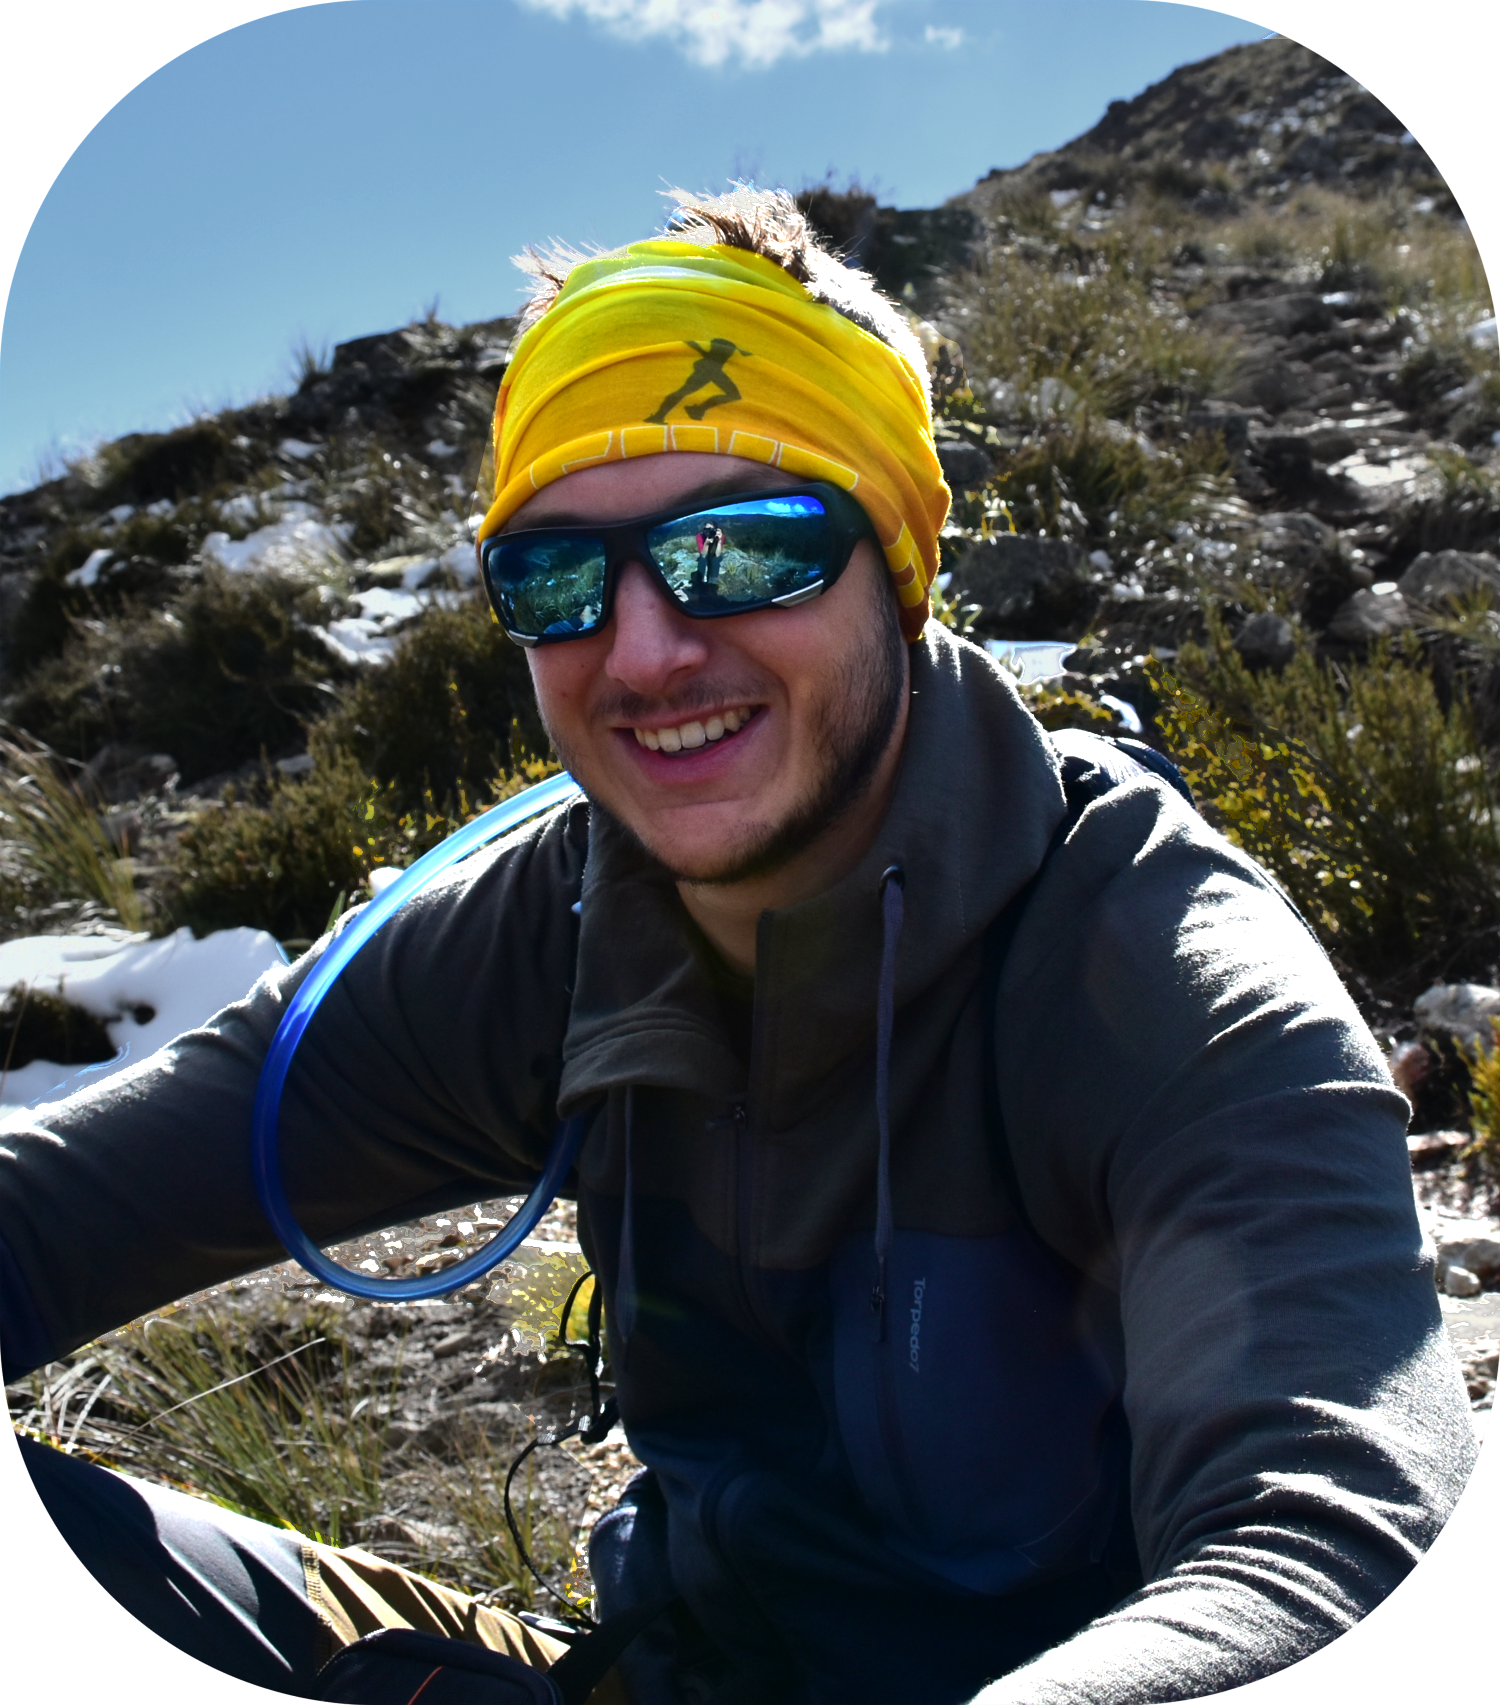
\includegraphics[width=3.5cm]{img/profile_relaxed.png}
  
\includegraphics[width=3.5cm]{img/QR.png}
  \section{Contact}
    \href{mailto:wesleybanfield@gmail.com}{\textbf{wesleybanfield@}\\gmail.com}
    ~
    +64 27 777 55 09
    ~
    25A Beckford Road,
    Christchurch, 8022
  \section{Web \& Git}
    \href{https://www.linkedin.com/in/wesleybanfield/}{Linkedin}
    \href{https://github.com/WesleyTheGeolien}{Github}
  % use  \hspace{} or \vspace{} to change bubble size, if needed
  \section{Technologies}
	\textbf{Jupyter}
\includegraphics[scale=0.40]{img/4stars.png}
	\textbf{Orange}
\includegraphics[scale=0.40]{img/4stars.png}
	\textbf{Plotly/Dash}
\includegraphics[scale=0.40]{img/4stars.png}
	\textbf{Sklearn}
\includegraphics[scale=0.40]{img/3stars.png}
	\textbf{Docker}
\includegraphics[scale=0.40]{img/3stars.png}
	\textbf{Microsoft PowerApps / Flow}
\includegraphics[scale=0.40]{img/2stars.png}
	~
  \section{Languages}
	\textbf{Python}
\includegraphics[scale=0.40]{img/5stars.png}
	\textbf{C++}
\includegraphics[scale=0.4]{img/3stars.png}
	\textbf{\LaTeX}
\includegraphics[scale=0.4]{img/4stars.png}
	~ 
	~
  \section{Geological Software}
	\textbf{LeapFrog}
\includegraphics[scale=0.40]{img/5stars.png}
	\href{http://www.ccgalberta.com/}{\textbf{CCG}}
\includegraphics[scale=0.40]{img/5stars.png}
	\href{http://www.pdgm.com/products/skua-gocad/}{\textbf{Skua}}
\includegraphics[scale=0.40]{img/3stars.png}
	\textbf{QGis}
\includegraphics[scale=0.40]{img/3stars.png}
	\href{https://snowdengroup.com/software/supervisor/}{\textbf{Supervisor}}
\includegraphics[scale=0.40]{img/3stars.png}
	~
%  \section{Personal Skills}
%    \smartdiagram[bubble diagram]{
%        \textbf{Team}\\\textbf{Player},
%        \textbf{Initiative},
%        \textbf{Curiosity},
%        \textbf{Problem}\\\textbf{Solving},
%        \textbf{\vspace{2mm}Manage\vspace{2mm}},
%        \textbf{Organize}
%    }
    ~
\end{aside}
~
\section{Experience}
\begin{entrylist}
  \entry
    {01/17 - Now}
    {Research Engineer}
    {\href{https://www.seequent.com/}{Seequent, Chirstchurch New Zealand}}
    {Regullarly called upon by key decsion makers to aide define the core stagegies of the company by providing technical expertise. A consderable amount of horizon 3 prototyping work is also carried out testing technical feasability and workflows.
    \\[6pt]
   	\textbf{New Technologies}
   	Infill Drilling, automatic drill hole hole error detection, Dashboard creation, Jupyter
   	\\[6pt]
   	\textbf{New Solutions}
   	Drilling Sensitivity analysis
    \\[6pt]
   	\textbf{Core stategy}
   	Processing metrics	
   	Krigin Validation
    \\[6pt]	
    \textbf{Infill drilling} conception of idea, implementation of backend, project coordination. Optimisation of where drilling needs to occur in mines to return most revenu with least cost. Cloud based processing set off from \href{https://www.lfview.com}{lfview}
    \\[6pt]
    \textbf{Drill hole sensitivity analysis} conception and implementation of workflow. Presentation of work, to clients, at \href{https://lyceum-perth.seequent.com/}{Perth Lyceum}. Creation of multiple models removing drill-holes and rebuilding implict model.
    \\[6pt]
    \textbf{Automatic drill hole error detection} Supervision of \href{https://www.canterbury.ac.nz/courseinfo/GetCourseDetails.aspx?course=SENG402\&occurrence=18W(C)\&year=2018}{SENG402} student. Chrome extension sets of machine learning algorithms in cloud deployed container.
    \\[6pt]
    \textbf{Processing metrics} Creation of infrastructure to extract, store and analyse key processing metrics of \href{https://www.leapfrog3d.com/}{Leapfrog}. Analysis of results to understand compute intensive tasks.
    \\[6pt]
    \textbf{Dashboard Creation} Implementation of web based dashboard solutions for groundwater monitoring. Collaboartion with \href{https://ecan.govt.nz/}{ECan} and \href{https://www.wrd.org/}{WRD, California}.
    \\
    Reference : \href{mailto:tim.schurr@seequent.com}{Tim Schurr, Solutions Architect}
	}
  \entry
    {05/16 - 19/16}
    {Software Integration Engineering Internship}
    {\href{https://www.total.com/en}{Total, Pau France}}
    {Interfacing with \href{http://www.ring-team.org/software/ringmesh}{RINGMesh} library for dynamic remeshing during coupled geomechanic - flow simulation workflows.\\ Reference : \href{mailto:tristan.cornu@total.com}{Tristan Cornu, Pore pressure and Rock Mechanics Specialist}}
    \entry
    {02/16 - 05/16}
    {Research Intern}
    {\href{http://www.ring-team.org/}{Ring Research Lab, Nancy France }}
    {Research and implementation of different automatic simultaneous well log correlation algorithms and creation of a SKUA-Gocad plugin, a program orginally developped in house before commercialisation by Paradigm. The work was presented and published in the 2016 Ring Meeting. \\Reference : \href{mailto:Guillaume.Caumon@ensg.univ-lorraine.fr}{Guillaume Caumon, Head of Research team}}
    \entry
    {06/15 - 09/15}
    {Software Engineering Internship}
    {\href{https://www.seequent.com/}{Seequent, Chirstchurch New Zealand}}
    {Design and development of a graphical user interface for geostatistical analysis in Leapfrog 3D Geological modelling suite, later integrated into Leapfrog EDGE. Implementation of different geostatistical algorithms.
    \\
    Reference : \href{mailto:tim.mclennan@seequent.com}{Tim McLennan}}
	\entry
	{09/14 - 05/15}
	{Lab Research Project}
	{\href{http://georessources.univ-lorraine.fr/}{GeoRessources, Nancy France}}
	{Oil age dating using Rhenium / Osmium. Designing experimental methods and analysing ICP MS results. 
	\\
	Reference : Raymond Michels}
\end{entrylist}
\\
\newpage

\begin{aside}
	~
	~
	~
	\section{OS Preference}
	\textbf{GNU/Linux}
\includegraphics[scale=0.40]{img/5stars.png}
	\textbf{Unix}
\includegraphics[scale=0.40]{img/4stars.png}
	\textbf{MacOS}
\includegraphics[scale=0.40]{img/2stars.png}
	\textbf{Windows}
\includegraphics[scale=0.40]{img/1stars.png}
	~
	\section{Places Lived}
	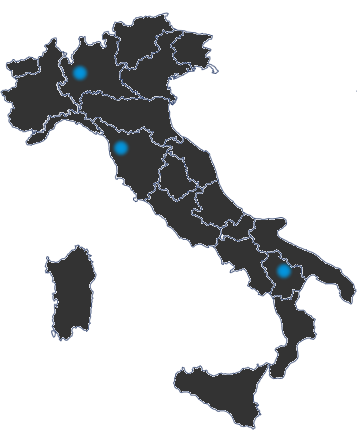
\includegraphics[scale=0.25]{img/italia.png}
	~
	\section{Languages}
	\textbf{Italian}
\includegraphics[scale=0.40]{img/5stars.png}
	\textbf{English}
\includegraphics[scale=0.40]{img/4stars.png}
	~
\end{aside}

\section{Education}
\begin{entrylist}
  \entry
    {2013 - 2016}
    {Masters in Geological Engineering with specialisation in Numerical Geology and Oil \& Gas Engineering}
    {\href{http://ensg.univ-lorraine.fr/english/}{French National School of Geological Engineering}}
    {Ecole National Superieur de Geologie is a leading French engineering school specialising in geosciences and delivering a 5 year University Diploma as well as a Masters from the University of Lorraine.\\ \emph{Curriculum}: Oil and Gas Engineering and Numerical Geolgy.\\ 
    \emph{Main subjects}: Structural Geology, Petroleum Systems, Sedimentology, Geomechanics, Mathematical concepts of geomodelling, Software Development, Interface Design, Computer Geometry, Visualisation and Parallelism, Finite Elements.\\
    \emph{Title of Thesis}: ”Current automatic well log correlation techniques, their advantages and drawbacks”.
    \emph{Relators}: Prof. Guillaume Caumon, Jonathan Edwards\\}
  \entry
    {2011 - 2013}
    {\href{https://en.wikipedia.org/wiki/Classe_preparatoire_aux_grandes_ecoles}{Classes Preparatoire aux Grandes Ecoles}}
    {Lycee Pierre de Fermat, Toulouse France}
    {2 years of intensive general scientific courses before national exams for entry to the French Grandes Ecoles, carried out in Pierre de Fermat, one of the top prep classes, 6 / 52\\ 
    \emph{Main subjects}: Geology, Matematics, Physics, Chemistry and Biology.\\}
\end{entrylist}

\newpage

\section{Publications}
Author, Author, Author\\
\textbf{Lorem ipsum dolor sit amet, consectetur adipiscing elit, sed do eiusmod tempor incididunt ut labore et dolore magna aliqua}\\
\emph{Lorem ipsum dolor sit amet, consectetur adipiscing elit, sed do eiusmod tempor incididunt ut labore et dolore magna aliqua}
\\
\section{Honors \& Awards}
\begin{entrylist}
  \entry
    {10/2015}
    {Best swordsman duel}
    {Contest}
    {Lorem ipsum.\\
    \emph{Lorem ipsum}}
\end{entrylist}

\section{Certifications}
\begin{entrylist}
  \entry
    {02/2013}
    {Intro to Computer Science}
    {Udacity. E-learning}
    {\emph{Building a Python Search Engine}}
\end{entrylist}

\section{Other Info}
For the Italian job market:\\
\emph{Si autorizza il trattamento delle informazioni contenute nel curriculum in conformità alle disposizioni previste dal d.lgs. 196/2003. Si dichiara altresì di essere consapevole che, in caso di dichiarazioni non veritiere, si è passibili di sanzioni penali ai sensi del DPR 445/00 oltre alla revoca dei benefici eventualmente percepiti.}
\\
\begin{flushleft}
\emph{May 8th, 2016}
\end{flushleft}
\begin{flushright}
\emph{John Snow}
\end{flushright}

\end{document}
